\documentclass[11pt]{article}

\usepackage[margin=1in]{geometry}
\usepackage{amsmath,amssymb,amsthm,mathtools}
\usepackage{enumitem}
\usepackage{hyperref}
\usepackage{graphicx}
\usepackage{booktabs}
\usepackage{verbatim}
\usepackage{caption}
\usepackage{subfig}
\usepackage{url}

\title{Machine Learning with Graphs: Homework II}
\author{Dev Sanghvi - ds221}
\date{Spring 2026}

\newcommand{\G}{G}
\newcommand{\R}{\mathbb{R}}

\begin{document}
\maketitle

\section*{Problem 1}

\begin{figure}[h]
\centering
\subfloat[$A$ is a true missing edge \label{fig::hw_2b1}]
{
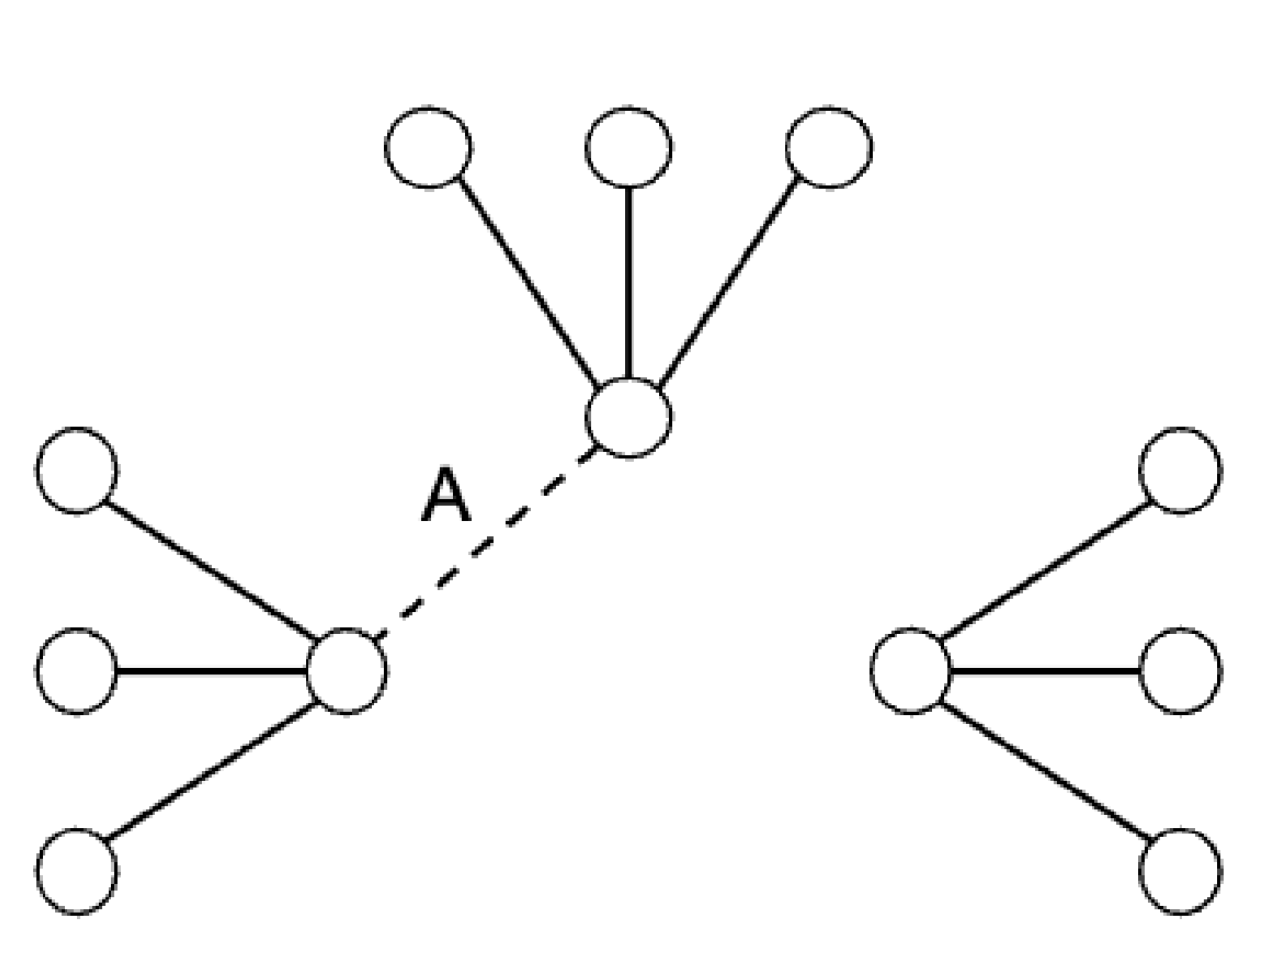
\includegraphics[keepaspectratio,width=.45\textwidth]{figures/1_a.png}
}
\qquad
\subfloat[$A$ and $B$ are true missing edges \label{fig::hw_2b2}]
{
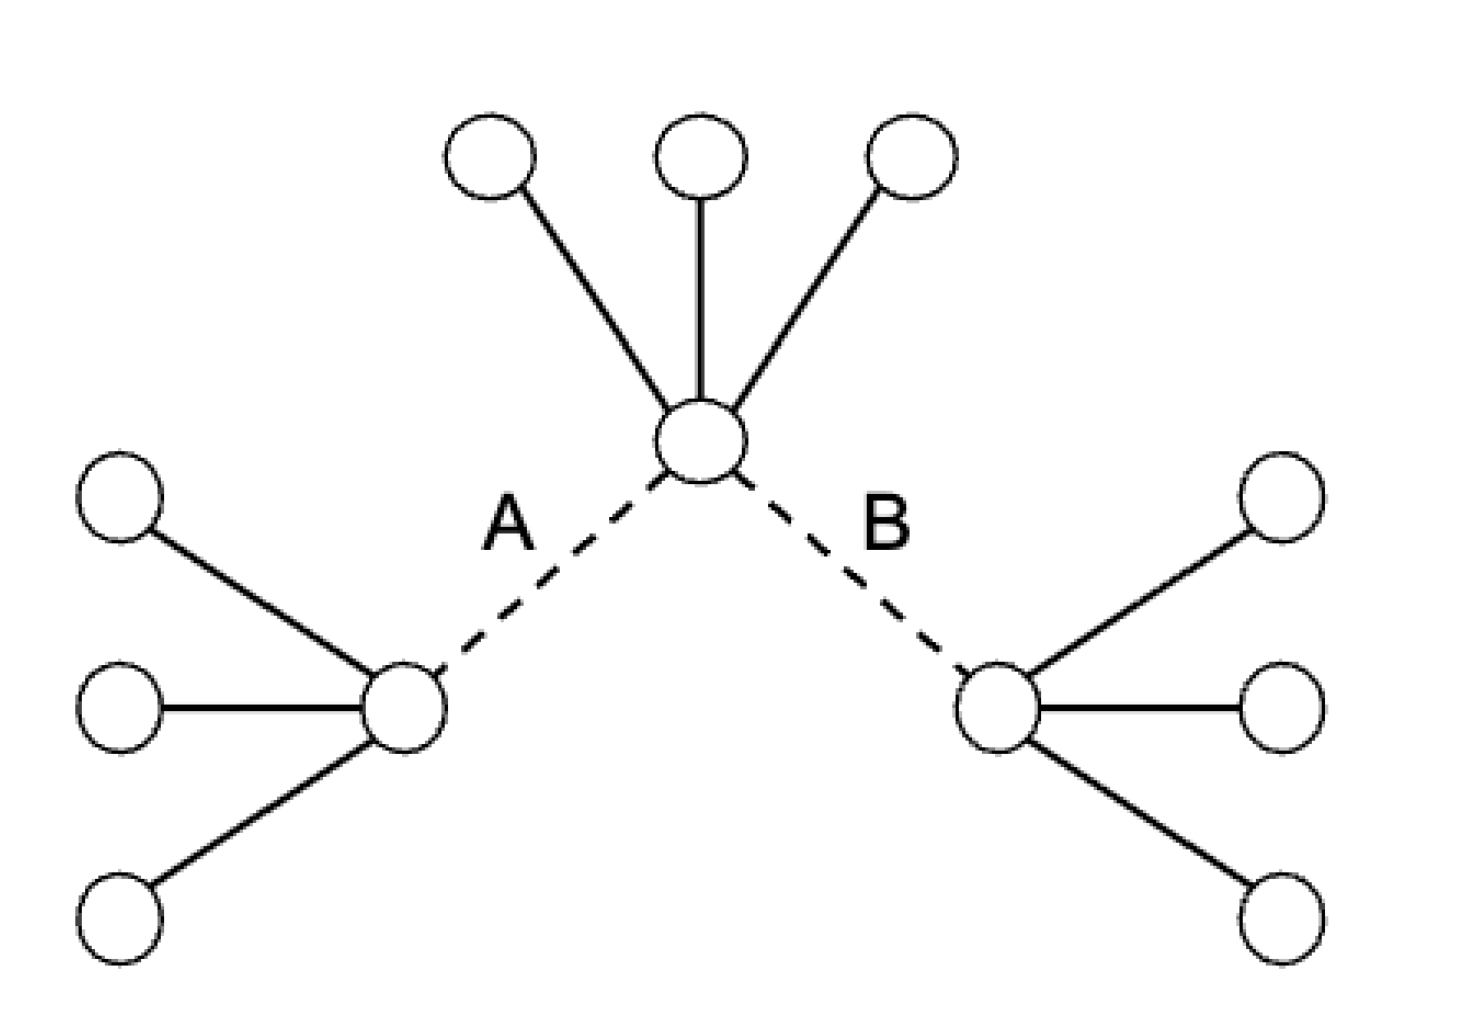
\includegraphics[keepaspectratio,width=.45\textwidth]{figures/1_b.png}
}
\caption{Problem 1 graphs.}
\end{figure}

\noindent Consider \textit{preferential attachment} score for link prediction, where an edge is predicted based on the degrees of its endpoints. The probability $p(u,v)$ of the edge $(u,v)$ is given as follows:
$$p(u,v) \propto \deg(u)\deg(v)$$

\paragraph{Task.}
Compute the AUC for preferential attachment using the graph from Figure \ref{fig::hw_2b1}, where $A$ is the only true missing edge. Do the same for the graph from Figure \ref{fig::hw_2b2}, where both $A$ and $B$ are true missing edges. Do these values reflect the difference in performance?

\paragraph{Solution.}
Based on the visual representation, we model the graph as three disconnected star components centered at hubs $L$, $T$, and $R$, each with 3 leaf nodes. The Preferential Attachment (PA) score for a potential edge $(u,v)$ is $PA(u,v) = \deg(u) \times \deg(v)$.
\begin{itemize}
    \item Hub-Hub edges (e.g., $L-T$, $T-R$, $L-R$) have score $3 \times 3 = 9$.
    \item Hub-Leaf edges have score $3 \times 1 = 3$.
    \item Leaf-Leaf edges have score $1 \times 1 = 1$.
\end{itemize}

\noindent \textbf{Evaluation Setup:} We define the candidate set for AUC calculation as \textit{all non-existing edges} in the graph. The goal is to rank the true missing edges (positive set) higher than all other non-edges (negative set).

\paragraph{Case (a): Target set is $\{A = (L, T)\}$.}
The target edge $A$ (Positive) has score $3 \times 3 = 9$.
We compare this against all 56 Negative non-edges.
\begin{itemize}
    \item \textbf{Negatives with Score 9:} There are 2 such edges: $(L,R)$ and $(T,R)$. Since Score(Pos) = Score(Neg), these count as 0.5 correct each. Contribution: $2 \times 0.5 = 1.0$.
    \item \textbf{Negatives with Score 3:} There are 18 such edges (Hub-Leaf non-edges). $9 > 3$, so these are correctly ranked. Contribution: $18 \times 1.0 = 18.0$.
    \item \textbf{Negatives with Score 1:} There are 36 such edges (Leaf-Leaf non-edges). $9 > 1$, so these are correctly ranked. Contribution: $36 \times 1.0 = 36.0$.
\end{itemize}
Total Correct Pairs = $1.0 + 18.0 + 36.0 = 55.0$.
$$ AUC = \frac{\text{Total Correct}}{\text{Total Negatives}} = \frac{55}{56} \approx 0.9821 $$
\textbf{Calculated AUC:} $0.9821$

\paragraph{Case (b): Target set is $\{A = (L, T), B = (T, R)\}$.}
We have 2 Positive edges ($A, B$) both with Score 9.
We compare these against the remaining $57 - 2 = 55$ Negative non-edges.
\begin{itemize}
    \item \textbf{Negatives with Score 9:} There is 1 such edge: $(L,R)$.
    Comparison with 2 Positives: $2 \times 0.5 = 1.0$ (Ties).
    \item \textbf{Negatives with Score 3:} There are 18 such edges.
    Comparison with 2 Positives: $2 \times 18 \times 1.0 = 36.0$ (Wins).
    \item \textbf{Negatives with Score 1:} There are 36 such edges.
    Comparison with 2 Positives: $2 \times 36 \times 1.0 = 72.0$ (Wins).
\end{itemize}
Total Correct Pairs = $1.0 + 36.0 + 72.0 = 109.0$.
Total Pairs = $2 \times 55 = 110$.
$$ AUC = \frac{109}{110} = 0.990909\dots \approx 0.9909 $$
\textbf{Calculated AUC:} $0.9909$

\paragraph{Conclusion.}
The AUC values (0.9821 vs 0.9909) do reflect a slight difference, but they are misleadingly high. The metric is dominated by the vast majority of easy-to-classify negative edges (e.g., Leaf-Leaf pairs with low degree product).
In Case (a), the true missing edge $A=(L,T)$ is tied for first place with two false positives ($(L,R)$ and $(T,R)$). A strict top-$k$ ranking metric would reveal this ambiguity better than AUC.
Therefore, a better alternative would be Hits@k (with $k=3$) or Mean Reciprocal Rank (MRR), which focus on the rank of the true positive among the highest-scoring candidates rather than the global discrimination against all negatives.

\paragraph{Comparison with Common Neighbors.}
Common Neighbors (CN) fails in this scenario.
The following calculation uses the setup from Case (a) (1 Positive, 56 Negatives), though the result is similar for Case (b).
Total Negatives = 56.
\begin{itemize}
    \item \textbf{False Positives (Score 1):} Any pair of leaves attached to the same hub shares that hub as a common neighbor. There are $\binom{3}{2} \times 3 = 9$ such pairs. Since $1 > 0$ (True Positive Score), these are ranked incorrectly.
    \item \textbf{True Positives (Score 0):} The missing edges connect two different hubs (e.g., $L$ and $T$), which share no common neighbors ($CN=0$).
    \item \textbf{True Negatives (Score 0):} The remaining $56 - 9 = 47$ non-edges have score 0. These are tied with the True Positive.
    \item \textbf{AUC Calculation:}
    $$ AUC = \frac{0.0 \times 9 + 0.5 \times 47}{56} = \frac{23.5}{56} \approx 0.4196 $$
\end{itemize}
Since $AUC < 0.5$, the CN predictor is performing worse than random guessing for ranking the missing links, making PA the superior choice.

\newpage
\section*{Problem 2 (optional)}

\begin{figure}[h]
\centering
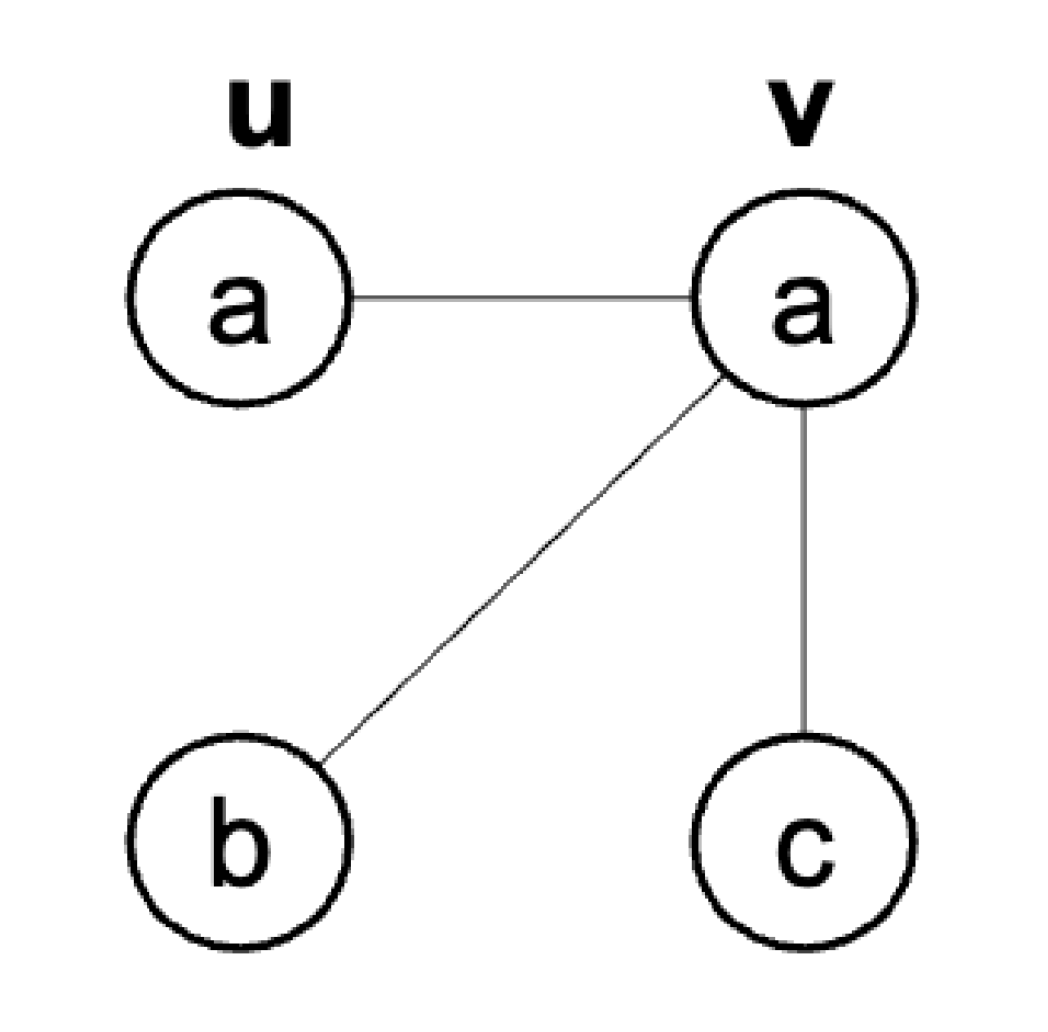
\includegraphics[keepaspectratio,width=.3\textwidth]{figures/2.png}
\caption{Problem 2 multiset example. \label{fig::problem2}}
\end{figure}

\noindent Consider a node classification model for attributed graphs where each node has a single attribute. For each node $v$, we collect the multiset of attributes within one hop from $v$ (i.e., $v$ and its neighbors). We generate vector representations in $\mathbb{R}^D$ for each vertex to represent its multiset. Use $\ell$ for possible attributes.

\subsection*{(a) Number of possible multisets}

\paragraph{Question.}
Given $\ell$ possible attributes, what is the number of possible multisets for a node with degree $d$?

\paragraph{Solution.}
This is a problem of counting combinations with replacement (multisets). For a node $v$ with degree $d$, the multiset contains $k = d+1$ attributes (itself plus $d$ neighbors), drawn from $\ell$ possible types.
The number of such multisets is given by the multiset coefficient:
$$ M_d = \binom{\ell + k - 1}{k} = \binom{\ell + d}{d+1} $$

\subsection*{(b) Dimensions for 32-bit representation}

\paragraph{Question.}
Assuming that each floating point in the (embedding) vector has 32 bits, how many dimensions are needed to represent these multisets?

\paragraph{Solution.}
To uniquely represent $M_d$ distinct multisets, we need $\lceil \log_2(M_d) \rceil$ bits of information.
Since each floating point number has 32 bits, the number of dimensions $D$ required is given by the total bits divided by 32, rounded up:
$$ D = \left\lceil \frac{\log_2(M_d)}{32} \right\rceil = \left\lceil \frac{\log_2 \binom{\ell + d}{d+1}}{32} \right\rceil $$

\subsection*{(c) Barabasi-Albert Model Simulation}

\paragraph{Question.}
If the graph is generated using the Barabasi-Albert model with each new node connecting to $c=5$ existing nodes, $n \to \infty$, and $\ell=100$, what would be a good estimate of the expected number of dimensions needed to represent at least half of the nodes? And to represent 99\% of the nodes? And to represent all the nodes?

\paragraph{Solution.}
Since $n \to \infty$, we must use the asymptotic degree distribution of the Barabasi-Albert model with parameter $m=5$. The degree distribution follows a power law with exponent $\gamma=3$:
$$ P(k) = \frac{2m(m+1)}{k(k+1)(k+2)} $$
For $m=5$, this becomes $P(k) = \frac{60}{k(k+1)(k+2)}$.
Based on the cumulative distribution function (CDF), we determine the degree thresholds.

\begin{itemize}
    \item \textbf{For 50\% of the nodes:}
    We sum $P(k)$ starting from $k=m$ until the cumulative probability exceeds 0.5.
    \begin{align*}
        P(5) &= \frac{60}{5(6)(7)} = \frac{60}{210} \approx 0.2857 \\
        P(6) &= \frac{60}{6(7)(8)} = \frac{60}{336} \approx 0.1786 \\
        P(7) &= \frac{60}{7(8)(9)} = \frac{60}{504} \approx 0.1190
    \end{align*}
    Sum: $0.2857 + 0.1786 + 0.1190 = 0.5833 > 0.5$.
    Thus, the threshold is $d_{50\%} = 7$.
    The number of possible multisets for $d=7$ is $M_{7} = \binom{100+7}{8} \approx 3.26 \times 10^{11}$.
    Dimensions required:
    $$ D_{50\%} = \left\lceil \frac{\log_2(3.26 \times 10^{11})}{32} \right\rceil = \left\lceil \frac{38.2}{32} \right\rceil = 2 $$

    \item \textbf{For 99\% of the nodes:}
    We need $\sum_{k=5}^{K} P(k) \ge 0.99$, which means the tail probability $\sum_{k=K+1}^{\infty} P(k) \le 0.01$.
    Using the continuous approximation for the tail of the power law $P(k) \approx 2m^2 k^{-3}$:
    $$ \int_{K}^{\infty} 2m^2 x^{-3} dx = \left[ -m^2 x^{-2} \right]_{K}^{\infty} = \frac{m^2}{K^2} $$
    Setting $\frac{25}{K^2} \le 0.01 \Rightarrow K^2 \ge 2500 \Rightarrow K \ge 50$.
    Exact numerical summation of the formula $P(k) = \frac{60}{k(k+1)(k+2)}$ confirms that $\sum_{k=5}^{54} P(k) \approx 0.9903 > 0.99$.
    Thus, $d_{99\%} = 54$.
    $$ M_{54} = \binom{100+54}{55} \approx 2.61 \times 10^{42} $$
    Dimensions required:
    $$ D_{99\%} = \left\lceil \frac{\log_2(2.61 \times 10^{42})}{32} \right\rceil = \left\lceil \frac{140.9}{32} \right\rceil = 5 $$

    \item \textbf{For all the nodes:}
    As $n \to \infty$, the maximum degree $d_{\max}$ scales as $d_{\max} \sim n^{1/(\gamma-1)} = n^{1/2}$ (derived from $\int_{d_{\max}}^\infty P(k)dk \approx 1/n$).
    Consequently, $M_d$ grows without bound, and the dimensions $D \sim \log(M_d)$ grow logarithmically. No finite $D$ suffices for the infinite limit, but for any finite $n$, $D$ is small.
\end{itemize}

\end{document}
